\subsection{Baselines, Code, and Material Provided} \label{sec:baselines}

\paragraph{Preliminary Baselines}

\begin{figure}
    \begin{center}

        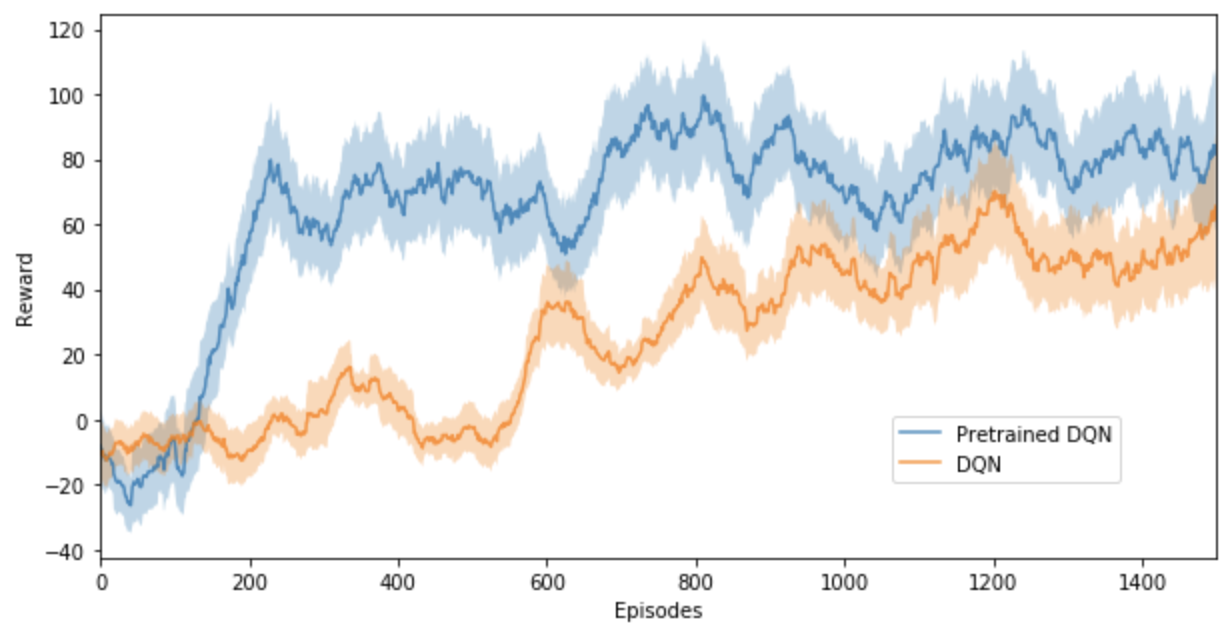
\includegraphics[width=0.49\textwidth]{./assets/dqn.png} 
        \caption{\small Performance graphs over time with DQN and PreDQN on \texttt{Navigate}(Dense)}
        \label{fig:dqn}

    \end{center}
\end{figure}

We present preliminary results showing the usefulness of the data for improving sample efficiency and overall performance. 
We compare algorithms by the highest average reward obtained over a 100-episode window during training.
We also report the performance of random policies and 50th percentile
human performance.
The results are summarized in Table~\ref{table:perf}.

In the presented comparison, DQN is an implementation of Double Dueling DQN~\cite{hasselt2015deep} and Behavioral Cloning is a supervised learning method trained on expert trajectories.
PreDQN denotes a version of DQN pretrained on the \minenet{}-v0 data: specifically, PreDQN is trained by performing Bellman updates on minibatches drawn from expert trajectories with accompanying reward labels. Before training, we initialize the replay buffer with expert demonstrations.

In all environments, the learned agents perform significantly worse than humans.
 \texttt{Treechop} exhibits the largest difference: on average, humans achieve a score of 64, but reinforcement agents achieve scores of less than 4. 
These results suggest that our environments are quite challenging, especially given that the \texttt{Obtain<Item>} environments build upon the Treechop environment by requiring the completion of several additional sub-goals.
We hypothesize that a large source of difficulty stems from the environment’s inherent
long-horizon credit assignment problems.
For example, it is hard for agents to learn to navigate through water because it
takes many transitions before the agent dies by drowning.

In light of these difficulties, our data is useful in improving performance and sample efficiency:
in all environments, methods that leverage human data perform better.
As seen in Figure~\ref{fig:dqn}, the expert demonstrations were able to achieve higher
reward per episode and attain high performance using fewer samples.
Expert demonstrations are particularly helpful in environments where random exploration 
is unlikely to yield any reward, like Navigate (Sparse). These preliminary results indicate that human demonstrations will be crucial in solving the main competition environment.



\begin{table}
    \small
    \centering
            \begin{tabular}{lccc}
                \toprule
                  & \texttt{Treechop} & \texttt{Navigate} (S) & \texttt{Navigate} (D) \\
                  \midrule
                 DQN \cite{mnih2015human}& 3.73 $\pm$ 0.61 & 0.00 $\pm$ 0.00 & 55.59 $\pm$ 11.38 \\
                 A2C \cite{mnih2016asynchronous}& 2.61 $\pm$ 0.50 & 0.00 $\pm$ 0.00 & -0.97 $\pm$ 3.23 \\
                 Behavioral Cloning & \textbf{43.9} $\pm$ \textbf{31.46} & 4.23 $\pm$ 4.15 & 5.57 $\pm$ 6.00 \\
                PreDQN & {4.16} $\pm$ {0.82} & {6.00} $\pm$ \textbf{4.65} & \textbf{94.96} $\pm$ \textbf{13.42} \\
                \midrule
                Human & 64.00 $\pm$ 0.00 & 100.00 $\pm$ 0.00 & 164.00 $\pm$ 0.00 \\
                Random & 3.81 $\pm$ 0.57 & 1.00 $\pm$ 1.95 & -4.37 $\pm$ 5.10 \\
                \bottomrule
            \end{tabular}
    \caption{
        \small Results in \texttt{Treechop}, \texttt{Navigate} (S)parse, and \texttt{Navigate} (D)ense, over the best 100 contiguous episodes. $\pm$ denotes standard deviation. 
        Note: humans achieve the maximum score for all environments shown.
    }
    \label{table:perf}
    \vspace{0pt}
\end{table}

\paragraph{2019 Baselines} 
For the 2019 MineRL Competition, Preferred Networks\footnote{\url{https://preferred.jp/en/}} provided extensive baselines\footnote{\url{https://github.com/minerllabs/baselines}}, including behavioral cloning, deep Q-learning from demonstrations (DQfD)~\citep{hester2018deep}, Rainbow~\citep{hessel2018rainbow}, generative adversarial inverse RL (GAIL)~\citep{gail_2016}, and proximal policy optimization (PPO)~\citep{ppo}. 
These baselines are implemented using ChainerRL~\cite{fujita2019chainerrl}, and MineRL 2019 participants found them to be incredibly helpful for developing their algorithms.
These baselines\footnote{Preferred Network's writeup of their experiments using their baselines and the MineRL environments can be found~\href{https://github.com/minerllabs/baselines/tree/master/general/chainerrl}{here}.} are available to participants to freely use in this iteration of the competition.

\paragraph{2020 Baselines}
We have again partnered with Preferred Networks to produce high-quality baselines. This year, the baselines are implemented using PyTorch~\cite{pytorch}.
These baselines consist of state-of-the-art RL and imitation learning algorithms, including Rainbow, SQIL~\cite{reddy2019sqil}, prioritized dueling double DQN (PDF DQN)~\cite{schaul2015prioritized,van2016deep,wang2016dueling}, and DQfD.
These baselines fully comply with the rules of this year's competition.

In addition to these baselines, we provide the code from the 2019 baselines and the top teams of the MineRL 2019 competition. 
However, these solutions do not conform to the rules of this year.
We hope competitors will be able to take inspiration from these methods.

\paragraph{Starting Code and Documentation.}
We released an open-source Github repository with starting code including the baselines mentioned above,
an OpenAI Gym interface for the Minecraft simulator, and a data-loader to accompany the data. 
Additionally, we released a public Docker container for ease of use.
We also provide participants with the code for the solutions from last year's top participants.
